% 抛物线 y^2=p(x+1)、直线 x+y=m 与 OQ、OR 示意；本图取 p=1、m=-0.8（满足 m>-1-p/4），
% 仅示关系，不按比例；Q 在上支左侧、R 在下支近轴，与源图同侧。
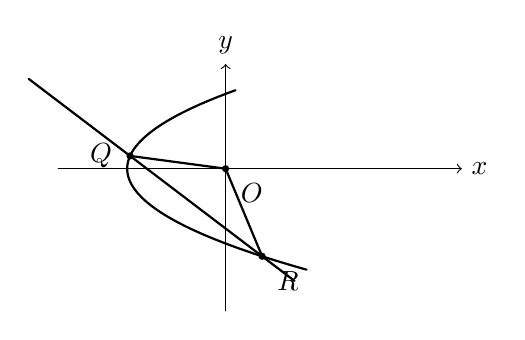
\begin{tikzpicture}[x=1.25cm,y=0.95cm,line cap=round,line join=round]
  \draw[->] (-1.7,0)--(2.4,0) node[right] {$x$};
  \draw[->] (0,-1.9)--(0,1.4) node[above] {$y$};
  \draw[thick,domain=-1.35:1.05,samples=100] plot ({\x*\x-1},{\x});
  \draw[thick,domain=-1.5:1.2,samples=60] plot ({-0.8-\x},{\x});
  \draw[thick] (0,0)--(-0.971,0.171);
  \draw[thick] (0,0)--(0.371,-1.171);
  \fill (0,0) circle (1.3pt) node[below right=2pt] {$O$};
  \fill (-0.971,0.171) circle (1.3pt) node[left=3pt] {$Q$};
  \fill (0.371,-1.171) circle (1.3pt) node[below right=2pt] {$R$};
\end{tikzpicture}
